
\section{Network Architecture}

Neural networks are often difficult to interpret due to complex interactions between multiple non-linear terms in their hidden layers. While it is easy to visualize curves in one or two dimensions, higher dimensional non-linearities quickly become confusing. By removing these joint interactions from the network, we can improve interpretability while only sacrificing a fraction of the network’s predictive power.

Our architecture consists of $n$ parallel sub-networks joined by an additive layer with sigmoid activation. Each sub-network has one input, one output, and one hidden layer containing $m$ sigmoid activated nodes. The output of these sub-networks represent the delinearization of each of the input variables. Each non-linearity is independent and can be plotted in two-dimensions.

\begin{figure}
    \centering
    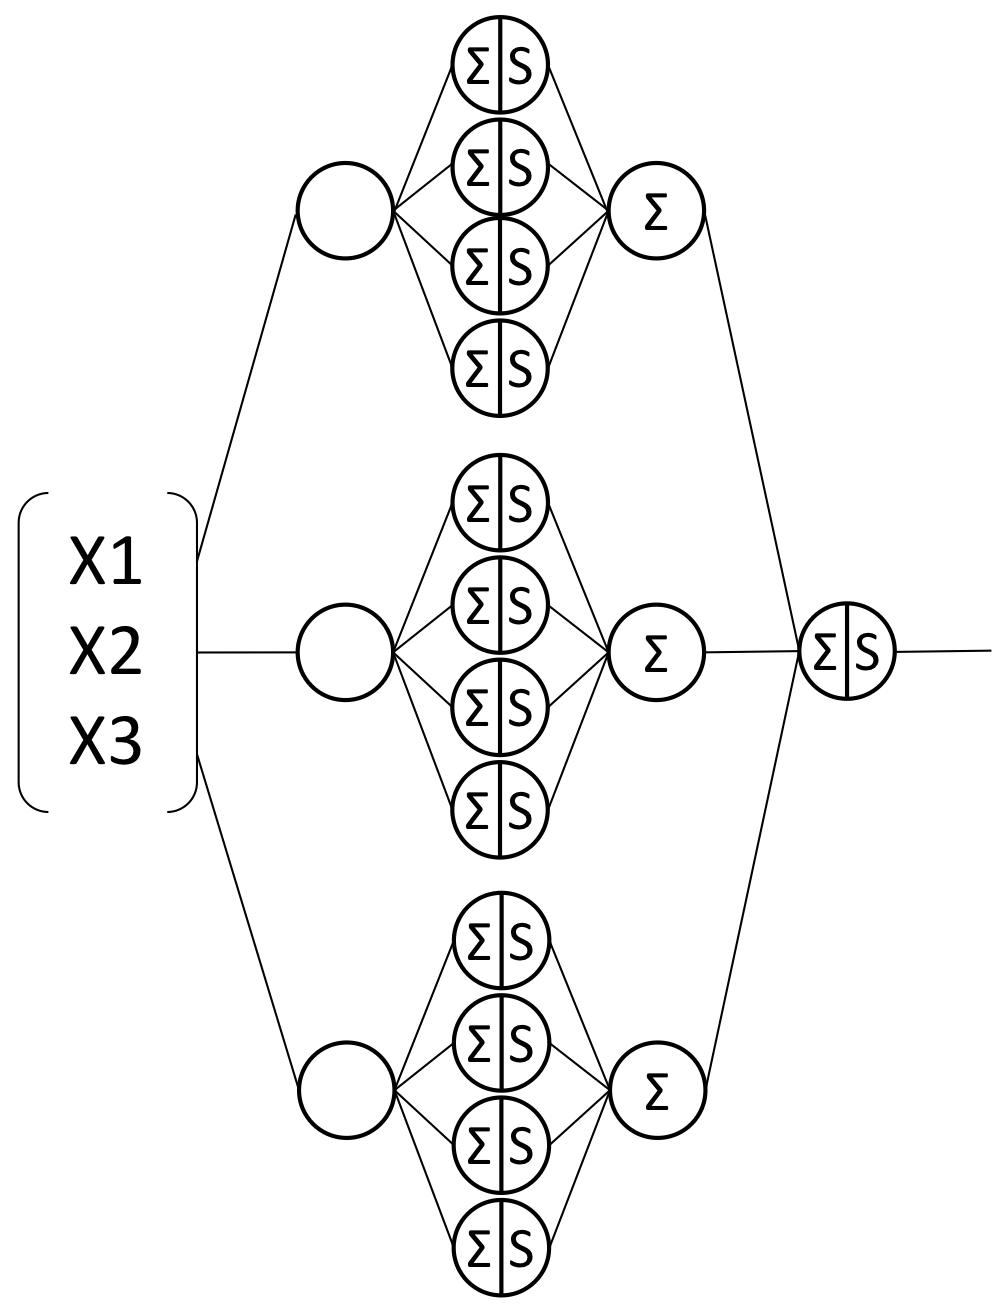
\includegraphics[width=0.65\textwidth]{fig/mnn}
    \caption{Example of our network architecture with n = 3 and m = 4. S represents a sigmoid activation.}
\end{figure}

Conceptually, this network works in three steps. First, the sub-networks delinearize each of the inputs, mapping the initial values $x$ to the more useful non-linear space $x'$. Second, the network weights each of the transformed $x'$ values according to vector $w$ and sums them together with a bias to generate score $y$. Third, $y$ is passed through a sigmoid activation function (logistic function with steepness 1) to realize the bounded classification $y'$. 

\begin{equation}
    \label{eq:network}
    y'_{net} = g(f_1(w_1 x_1) + f_2(w_2 x_2) + ... + f(w_n x_n))
\end{equation}

In theory, this methodology is identical to a GAM with b-splines and a sigmoid link function. \update{In practice however, the sigmoid activations of the neural network can actually fit a wider range of one-dimensional functions than the b-spline GAM. Whereas the GAM is restricted to the polynomial-like equations defined by its splines, the neural network can allocate its hidden units to different regions of the input space. This feature gives the network more flexibility in its approximations, which can result in improved performance (see experiment 2).}

We implemented our network in Keras \citep{Chollet2019Keras} using an Adam optimizer \citep{Kingma2014Adam:Optimization} with a learning rate of 0.1. The number of marginal networks is always equivalent to the number of input variables. Each marginal network has one input, one output, and contains one hidden layer with eight sigmoid-activated hidden units. The outputs of the marginal networks are combined in a final dense layer with sigmoid activation.

\section{Hypotheses}

\paragraph{H1.} \update{Our network architecture is interpretable and will closely approximate GAM behavior.}

\paragraph{H2.} Our network architecture will outperform b-spline GAMs in real-world datasets where the optimal non-linearity is unimodal with high variance over a small domain. 

\paragraph{H3.} Our network architecture will fail on classification problems where joint terms are required, such as the XOR problem. 

\paragraph{H4.} \update{Our network architecture will outperform logistic regression in all tested real-world classification datasets.}

\paragraph{H5.} Our network architecture will approach, but not surpass, the performance of GBMs on any tested real-world dataset. 

\paragraph{H6.} Our network architecture can be combined with deep networks to form more interpretable models in deep learning tasks. 

%\paragraph{H6.} Our network architecture will perform better on classification problems than regression problems. 


\section{Datasets}

\subsection{Real World}

To demonstrate the effectiveness of our architecture in real-world classification problems, we compare our method to standard techniques on a number of \update{common benchmark datasets. All datasets in this section have been well-studied in machine learning literature and were selected to represent a wide range of sample and feature space sizes. While our network architecture can be used in multi-class classification tasks, to standardize our comparison, we convert all non-binary classification datasets to binary classification problems by selecting the most difficult class to separate.}

In all experiments, the data is randomly shuffled before being fed in to the model. We use 50\% of the available data for training and 20\% of the available data for validation. \update{A simple grid search is used to determine the best hyper-parameters for each model. The model is then refit on the combined training and validation data} and test results are reported over the remaining 30\%.

\paragraph{Wisconsin Breast-Cancer Dataset:} \citep{Street2005NuclearDiagnosis} The Wisconsin breast cancer dataset contains 569 observations of 31 features that are used to predict if a given tumor is malignant or benign. There are 212 malignant and 357 benign examples in the dataset. Feature examples include the tumor's mean texture, radius, and perimeter. The response is not linearly separable given the input features. 

\paragraph{Sloan Sky Survey:} \citep{Blanton2017SloanUniverse} The Sloan Sky Survey dataset contains 10,000 examples of 17 features used to predict if a given celestial object is a star, galaxy, or quasar. The dataset contains 4998 examples of galaxies, 4512 examples of stars, and 850 examples of quasars. Example features include red-shift, ascension angle, and u-band magnitudes. \update{We reduce this dataset to a binary classification task by separating galaxies from other celestial objects.}

\paragraph{Iris:} \citep{Fisher1936TheProblems} Iris is a famous dataset comparing different species of the Iris plant. It contains 150 observations of four input variables: sepal length, sepal width, petal length, and petal width. The objective is to correctly classify 50 examples of Iris setosa, Iris versicolor, and Iris virginica using the four input features. In our experiments, we converted this problem from a multi-class classification problem to a single-class classification problem by trying to separate Iris versicolor from the other two classes. 

\paragraph{Titanic:} \citep{Stanford2019AProbability} The Titanic dataset contains 1309 rows corresponding to the passengers who were on board the Titanic the night it sank. The objective is to use the 13 input features to predict which passengers survived and which ones died during the disaster. Feature examples include sex, age, and ticket fare. 500 passengers survived the wreck while 809 perished. 

\paragraph{Wine:} \citep{Forina1991UCISet} \update{The wine dataset contains 178 instances of 13 variables corresponding to the attributes of different Italian wine samples. The original dataset contains 59, 71, and 48 examples of each of the output classes. We simplify this dataset to a binary classification task by taking the class with the most intermediate values in the first principle component.}


\subsection{Synthetic}

In experiment 3, we employ several synthetic datasets to demonstrate the theoretical limitations of the GAM approach. These datasets are as follows. 

\paragraph{Gaussian Islands:} The Gaussian Islands are two synthetic datasets, \textit{circle} and \textit{ellipse}, containing 2000 observations of two features bounded between positive and negative five. A two-dimensional Gaussian distribution with mean of zero and variance of one is placed in the center of each grid. In the circle dataset, the covariance between $x_1$ and $x_2$ is zero while in the ellipse dataset, the covariance is 0.5. Each observation is randomly placed on the grid. If the value of the Gaussian distribution at that point is greater than one, the point is considered a true positive, if the value is less than one, the point is a true negative. 

\begin{figure}
\centering
\begin{subfigure}{.5\textwidth}
  \centering
  \includesvg[width=0.9\linewidth]{fig/circle.svg}
  \caption{Gaussian island with covariance of 0.0.}
\end{subfigure}%
\begin{subfigure}{.5\textwidth}
  \centering
  \includesvg[width=0.9\linewidth]{fig/ellipse.svg}
  \caption{Gaussian island with covariance of 0.5.}
\end{subfigure}
\caption{Training data for the simulated Gaussian Islands dataset. Blue points are true positives, red points are true negatives.}
\label{fig:gaussian_islands}
\end{figure}

\paragraph{Simulated XOR:} \citep{Hara2016MakingInterpretable} The simulated XOR dataset contains 2000 randomly selected observations of two features bounded between positive and negative five. If the product of the features is positive, the point is a true positive, if negative, the point is a true negative. 

\begin{figure}[ht]
\caption{Training data for the simulated XOR dataset. Blue points are true positives, red points are true negatives.}
\includesvg[width=0.65\textwidth]{fig/xor.svg}
\label{fig:xor}
\centering
\end{figure}

\subsection{Pandemic}

Pandemic is a novel image classification benchmark involving a fictional disease modeled on Yersinia pestis: the bacteria responsible for the black plague \citep{Perry1997YersiniaPlague.}. It is designed as a simple synthetic benchmark for our architecture in image classification tasks.

Most highly contagious diseases tend to follow a common track when they encounter an uninfected individual. First, upon contact with the new host, the contagion rapidly begins to multiply in the favorable environment. The host's immune system identifies the threat and begins to take measures to mitigate the disease. One of these measures is to rapidly bolster t-cell production, a type of white blood cell that will actively fight the contagion. 

Depending on the severity of the disease and the frailty of the host, two outcomes are possible: the host's body mounts a rapid response and fights off the disease, or the contagion multiplies out of control, killing the host. These outcomes depend on how quickly the contagion multiplies and how quickly the body can produce an effective immune response. In our dataset, the immune response can be measured by proxy by taking a sample from an infection site and observing the relative frequencies of the bacteria and t-cells.

These samples consist of eight-hundred and seventy 120x120 black and white images containing a number of overlapping t-cells and bacteria. In these images, bacteria are modeled by a plus shape and t-cells are modeled by a square shape, as illustrated in Figure \ref{fig:pandemic_sample}. The total number of objects in any sample is bounded between zero and one-hundred. 

\begin{figure}
\centering
\begin{subfigure}{.5\textwidth}
  \centering
  \includesvg[width=0.9\linewidth]{fig/ex6/t_cell.svg}
\end{subfigure}%
\begin{subfigure}{.5\textwidth}
  \centering
  \includesvg[width=0.9\linewidth]{fig/ex6/bacterium.svg}
\end{subfigure}
\caption{Examples of a t-cell (left) and a bacterium (right) in the pandemic dataset.}
\label{fig:pandemic_sample}
\end{figure}

The distributions of t-cells and bacteria are governed by equations \ref{eq:s_t}, \ref{eq:i_t}, and \ref{eq:c_t}, represented graphically in Figures \ref{fig:pandemic_base_1} and \ref{fig:pandemic_base_2}. 

\begin{equation}
    \label{eq:s_t}
    s(t) = \frac{1}{1 + e^{-t}}
\end{equation}

\begin{equation}
    \label{eq:i_t}
    i(t) = s(t - c_i)
\end{equation}

\begin{equation}
    \label{eq:c_t}
    c(t) = s(v t - c_v) (1 - i(t))
\end{equation}

Ostensibly, both the t-cell and bacterial distributions are modeled as time-lagged sigmoids, representing an exponential ramp-up in production before tapering as the host reaches capacity. The bacterial distribution is scaled by one minus the t-cell \update{fraction}, representing how the immune system's ramp-up up allows the body to fight off the infection. 

Time-lag constants $c_i$ and $c_v$ are used to control the exact shape of the distributions, and for this experiment are set to one and three respectively. The viral rate $v$ is bounded between two and four, with all values above three being considered fatal.

\begin{figure}
    \includesvg[width=0.65\textwidth]{fig/ex6/pandemic_base_1.svg}
    \centering
    \caption{Plots of t-cell and bacteria distributions over time with $v = 3$. T-cell \update{fraction} increases throughout the simulation while the bacteria \update{fraction} peaks and then returns to zero.}
    \label{fig:pandemic_base_1}
\end{figure}


\begin{figure}
    \includesvg[width=0.65\textwidth]{fig/ex6/pandemic_base_2.svg}
    \centering
    \caption{Bacteria distributions with $v$ varying between two and four. Redder values correspond to higher values of $v$ and are considered to be more lethal.}
    \label{fig:pandemic_base_2}
\end{figure}

\update{While these classes are easy to separate as-is, the sampling complication described in the following section makes accurate classification much more difficult, if not impossible. Specifically, the sampling approach adds significant noise to the dataset, thereby overlapping the two tails of the distribution and destroying most of the non-linear behavior. Therefore, we introduce two minor changes to the distribution to achieve slightly greater separation between fatal and non-fatal cases.} First, we ignore all values $v$ between 2.75 and 3.25 and second, we add lift constant of 0.15 to all fatal cases. \update{Conceptually, this change removes the most difficult edge cases from the dataset and adds a small amount of bacteria to the fatal cases.}

A total of 870 samples are taken in grid fashion from this modified distribution by uniformly varying rate parameter $v$ and time parameter $t$ as shown in Figure \ref{fig:pandemic_sample_distribution}. \update{For testing, a new set of 870 images is generated from the same distribution.}

\begin{figure}
    \includesvg[width=0.65\textwidth]{fig/ex6/pandemic_sample_distribution.svg}
    \centering
    \caption{Final distribution of bacteria and t-cells from which we pull our image samples. Red x's are lethal while blue o's are non-lethal.}
    \label{fig:pandemic_sample_distribution}
\end{figure}

An image is generated for each sample by scaling outputs $i$ and $c$ by fifty times the inverse of the maximum value for each distribution (equations \ref{eq:ip_t} and \ref{eq:cp_t}). 

\begin{equation}
    \label{eq:ip_t}
    i'_t = \frac{50 i_t}{\max(i)}
\end{equation}

\begin{equation}
    \label{eq:cp_t}
    c'_t = \frac{50 c_t}{\max(c)}
\end{equation}

This step is a linear transformation that forces each of the values between zero and fifty. Objects are then added to the image in random locations with total frequencies corresponding to the transformed values $i'$ and $c'$. Finally, a layer of uniform noise is applied across the image. An example of this process is shown in Figure \ref{fig:pandemic_sample_images}.

\begin{figure}
    \centering
    \begin{subfigure}{.5\textwidth}
      \centering
      \includesvg[width=0.9\linewidth]{fig/ex6/image_10.svg}
    \end{subfigure}%
    \begin{subfigure}{.5\textwidth}
      \centering
      \includesvg[width=0.9\linewidth]{fig/ex6/image_50.svg}
    \end{subfigure}
    \caption{Example input images with 20 (left) and 100 (right) objects.}
    \label{fig:pandemic_sample_images}
\end{figure}

Intuitively, this dataset represents a two-part classification task where the model must first identify and count the number of each object in an image and then use those counts to classify it. While each task is relatively simple on its own, the combination of the two presents a more difficult hybrid challenge for most machine learning methods. The counting aspect requires image processing techniques, like convolutional networks, while the classification task requires a method with non-linear predictive power.

In this research, our objective is to correctly classify this dataset using a single model that is partially interpretable. \update{The rationale being that a single model is both easier to deploy in the field as well as trainable in a single step, due to the existence of a gradient over the custom layer.}

\update{While other datasets exist that could demonstrate this architecture, Pandemic provides two useful features for our analysis. First, every Pandemic sample has an explicit two-dimensional latent space (bacteria and t-cell counts) that is easy to understand and to visualize. Most image classification tasks require the development of an implicit latent space using a technique like auto-encoders} \citep{Baldi2012AutoencodersArchitectures}, \update{adding unnecessary complexity and obfuscation to our analysis. Second, the Pandemic image classification task is very simple, allowing the experiment to be run on less powerful hardware. While extensions of this methodology are applicable on many datasets, Pandemic is designed to be faster to run and easier understand for the purposes of this demonstration.}


\section{External Libraries}

\paragraph{PyGAM:} \citep{Serven2018PyGAM:Python} PyGAM is the leading implementation of generative additive models in Python. It provides support for standard and logistic GAMs, as well as built-in support for b-splines. In this work, PyGAM  is used as a baseline comparison for our neural network technique.

\paragraph{TensorFlow/Keras:} \citep{Chollet2019Keras} \citep{Allaire2019RTensorFlow} TensorFlow is an open source neural network development package developed by Google. It is one of the most powerful and widely used neural networks frameworks available today. Keras is an abstraction layer included in the base TensorFlow package which makes it easier to build and train neural networks. All neural networks presented in this paper were built in Keras with a TensorFlow back-end.

\paragraph{SciKit-Learn:} \citep{Pedregosa2011Scikit-learn:Python} SciKit-Learn is the de facto standard framework for machine learning in Python. It provides implementations for logistic regression, random forests, and gradient boosted machines, which are used as benchmarks and points of comparison for our model. 